\documentclass[12pt,english,nohyper]{tufte-handout}\usepackage[]{graphicx}\usepackage[]{color}
%% maxwidth is the original width if it is less than linewidth
%% otherwise use linewidth (to make sure the graphics do not exceed the margin)
\makeatletter
\def\maxwidth{ %
  \ifdim\Gin@nat@width>\linewidth
    \linewidth
  \else
    \Gin@nat@width
  \fi
}
\makeatother

\definecolor{fgcolor}{rgb}{0.345, 0.345, 0.345}
\newcommand{\hlnum}[1]{\textcolor[rgb]{0.686,0.059,0.569}{#1}}%
\newcommand{\hlstr}[1]{\textcolor[rgb]{0.192,0.494,0.8}{#1}}%
\newcommand{\hlcom}[1]{\textcolor[rgb]{0.678,0.584,0.686}{\textit{#1}}}%
\newcommand{\hlopt}[1]{\textcolor[rgb]{0,0,0}{#1}}%
\newcommand{\hlstd}[1]{\textcolor[rgb]{0.345,0.345,0.345}{#1}}%
\newcommand{\hlkwa}[1]{\textcolor[rgb]{0.161,0.373,0.58}{\textbf{#1}}}%
\newcommand{\hlkwb}[1]{\textcolor[rgb]{0.69,0.353,0.396}{#1}}%
\newcommand{\hlkwc}[1]{\textcolor[rgb]{0.333,0.667,0.333}{#1}}%
\newcommand{\hlkwd}[1]{\textcolor[rgb]{0.737,0.353,0.396}{\textbf{#1}}}%

\usepackage{framed}
\makeatletter
\newenvironment{kframe}{%
 \def\at@end@of@kframe{}%
 \ifinner\ifhmode%
  \def\at@end@of@kframe{\end{minipage}}%
  \begin{minipage}{\columnwidth}%
 \fi\fi%
 \def\FrameCommand##1{\hskip\@totalleftmargin \hskip-\fboxsep
 \colorbox{shadecolor}{##1}\hskip-\fboxsep
     % There is no \\@totalrightmargin, so:
     \hskip-\linewidth \hskip-\@totalleftmargin \hskip\columnwidth}%
 \MakeFramed {\advance\hsize-\width
   \@totalleftmargin\z@ \linewidth\hsize
   \@setminipage}}%
 {\par\unskip\endMakeFramed%
 \at@end@of@kframe}
\makeatother

\definecolor{shadecolor}{rgb}{.97, .97, .97}
\definecolor{messagecolor}{rgb}{0, 0, 0}
\definecolor{warningcolor}{rgb}{1, 0, 1}
\definecolor{errorcolor}{rgb}{1, 0, 0}
\newenvironment{knitrout}{}{} % an empty environment to be redefined in TeX

\usepackage{alltt}
\usepackage[T1]{fontenc}
\usepackage[utf8]{inputenc}
\usepackage{longtable}
\usepackage{wrapfig}
\usepackage{hyperref}
\usepackage{graphicx}
\usepackage[space]{grffile}
\usepackage{geometry}
\usepackage{pgffor}
%\usepackage{caption}
\usepackage{calc}
\usepackage{enumitem}
\usepackage{microtype}
%\usepackage{floatrow} % test for caption below
\usepackage{tabularx}
%\usepackage[capposition=bottom]{floatrow}
\IfFileExists{upquote.sty}{\usepackage{upquote}}{}
\begin{document}



\centerline{\Large\bf Statistics 101 Homework Short Report for Topic 04 AB}
\vspace{1cm}

\begin{marginfigure}
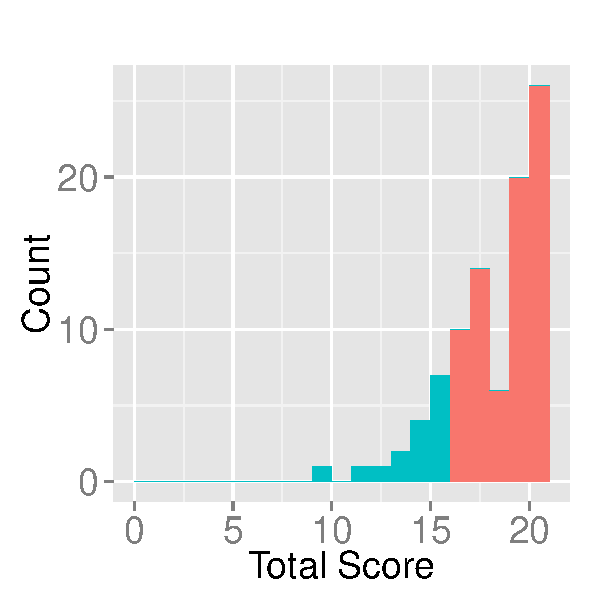
\includegraphics[width=0.98\linewidth]{Topic04_AB_score}
\caption{\label{mar:hist}Histogram of scores. Blue data represent scores less than 80 percent.}
\end{marginfigure}

Each of the 92 students were given 20 questions from a bank of 54 questions. Figure \ref{mar:hist} and Table \ref{tab:summary} give the overall summary of student performance. Table \ref{tab:studentsbelow80} lists the students who did not perform well on this homework. Table \ref{tab:QuestionSet_summary} and Figure \ref{fig:LearningObj_summary} provide summary statistics of the scores per question set and learning outcome.
\bigskip{}

% latex table generated in R 3.1.3 by xtable 1.7-4 package
% Fri Sep  4 12:31:53 2015
\begin{longtable}{llllllll}
  \hline
Mean & Std.dev &   & Min & Q1 & Median & Q3 & Max \\ 
  \hline
17.66 & 2.37 &  & 9.00 & 16.00 & 18.50 & 20.00 & 20.00 \\ 
  (88\%) & (12\%) &  & (45\%) & (80\%) & (92\%) & (100\%) & (100\%) \\ 
   \hline
\hline
\caption{Summary statistics of the scores} 
\label{tab:summary}
\end{longtable}




\begin{fullwidth}
\makeatletter\setlength\hsize{\@tufte@fullwidth}\makeatother
% latex table generated in R 3.1.3 by xtable 1.7-4 package
% Fri Sep  4 12:31:54 2015
\begin{longtable}{rr|lr|lr|lr}
  \hline
  & \% Correct &   & \% Correct &   & \% Correct &   & \% Correct \\ 
  \hline
adice & 75.00 & jtwalker & 75.00 & capeters & 70.00 & tbeatty & 65.00 \\ 
  akmorton & 75.00 & kives & 75.00 & grantsch & 70.00 & evan & 60.00 \\ 
  cds & 75.00 & nsevers & 75.00 & jwiltz17 & 70.00 & crmwoods & 55.00 \\ 
  jaeleaha & 75.00 & bergeson & 70.00 & jcanders & 65.00 & jng & 45.00 \\ 
   \hline
\hline
\caption{Students whose correct percentages are less than 80\%.} 
\label{tab:studentsbelow80}
\end{longtable}

\end{fullwidth}



\vspace{-2mm}

\noindent
\underline{Topic 04 Learning Outcomes:}
\vspace{2mm}

\begin{fullwidth}
\begin{enumerate}[label=\Alph*.,itemsep=-\parsep,leftmargin=*]
  \item
Identify various ways to describe the relationship between two categorical variables.
\item Describe the connection between the data table and the contingency table for summarizing the relationship between two categorical variables.
\item Identify the response and explanatory variables for investigating the relationship between two categorical variables.
\item Determine the marginal distributions of the two categorical variables from a contingency table.
\item Determine the conditional distributions or conditional proportions of the response variable given the explanatory variable from a contingency table.
\item Interpret displays of the relationship between two categorical variables to make generalizations within the context of the problem.
\item Determine whether or not there is an association between the response variable and the explanatory variable using a mosaic plot (segmented bar charts) or contingency table.

\end{enumerate}
\end{fullwidth}



\vspace{5mm}

%\begin{fullwidth} %ADDED NOW
%\makeatletter\setlength\hsize{\@tufte@fullwidth}\makeatother %ADDED NOW
%\begin{centering}
\begin{figure}[!ht]
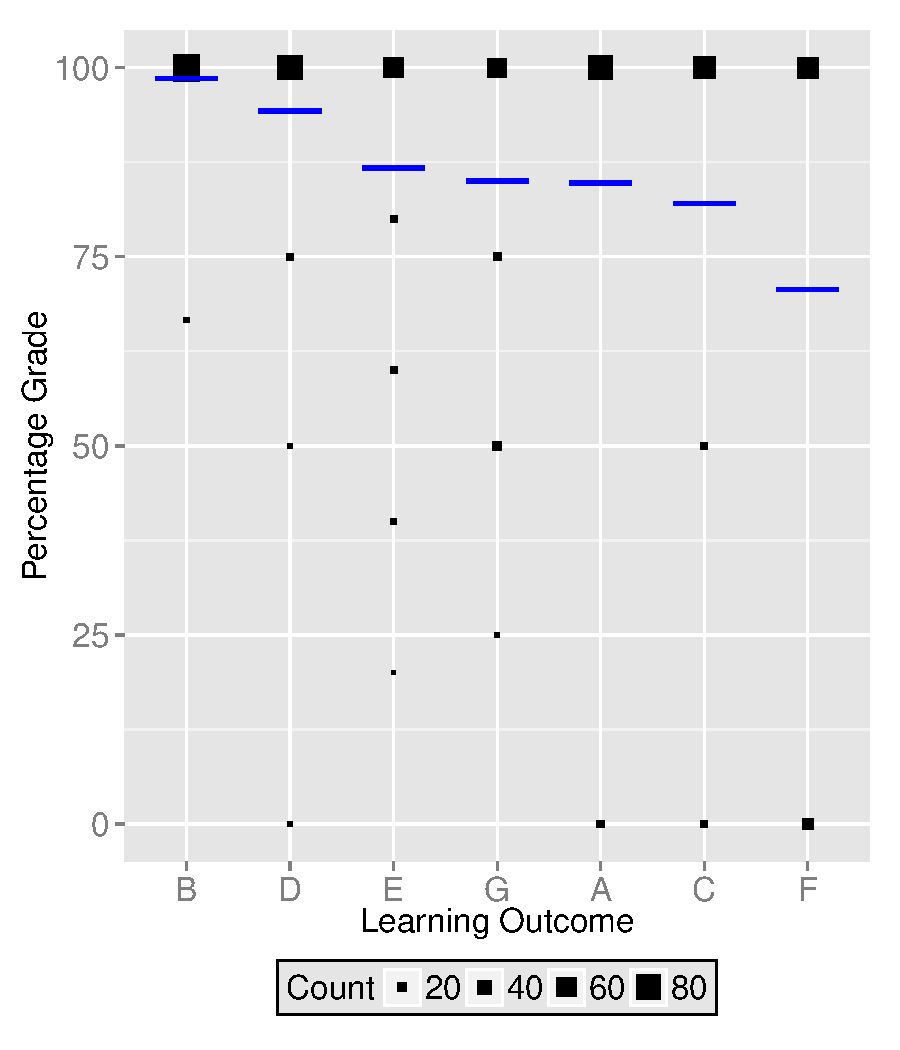
\includegraphics[width=\linewidth]{Topic04_AB_LearningObj_boxplot.pdf}
\caption{Fluctuation diagram of percentage correct by learning outcome. Mean scores are drawn as blue bars.}
\label{fig:LearningObj_summary}
\end{figure}
%\end{centering}
%\end{fullwidth} %ADDED NOW

\begin{fullwidth}
\makeatletter\setlength\hsize{\@tufte@fullwidth}\makeatother
% latex table generated in R 3.1.3 by xtable 1.7-4 package
% Fri Sep  4 12:31:54 2015
\begin{longtable}{cc|ccc|ccc}
  \hline
LO & Qset & \# & Mean & Std.dev & Min & Median & Max \\ 
  \hline
B & B &   4 & 100 & 0.00 & 100.00 & 100.00 & 100.00 \\ 
  B & D &   4 & 98.91 & 10.43 & 0.00 & 100.00 & 100.00 \\ 
  B & C &   4 & 96.74 & 17.86 & 0.00 & 100.00 & 100.00 \\ 
  G & L &   1 & 95.65 & 20.50 & 0.00 & 100.00 & 100.00 \\ 
  D & G &   5 & 95.11 & 19.70 & 0.00 & 100.00 & 100.00 \\ 
  D & F &   5 & 93.48 & 19.91 & 0.00 & 100.00 & 100.00 \\ 
  G & M &   1 & 93.48 & 24.83 & 0.00 & 100.00 & 100.00 \\ 
  E & I &  10 & 89.13 & 26.20 & 0.00 & 100.00 & 100.00 \\ 
  A & A &   2 & 84.78 & 36.12 & 0.00 & 100.00 & 100.00 \\ 
  E & H &   5 & 83.15 & 34.19 & 0.00 & 100.00 & 100.00 \\ 
  C & E &   5 & 82.07 & 34.44 & 0.00 & 100.00 & 100.00 \\ 
  G & K &   1 & \color{red}{78.26} & 41.47 & 0.00 & 100.00 & 100.00 \\ 
  G & N &   3 & \color{red}{72.83} & 44.73 & 0.00 & 100.00 & 100.00 \\ 
  F & J &   4 & \color{red}{70.65} & 45.79 & 0.00 & 100.00 & 100.00 \\ 
   \hline
\hline
\caption{Summary statistics of the question sets. Rows are sorted by mean scores, which are marked red if less than 80 percent.} 
\label{tab:QuestionSet_summary}
\end{longtable}

\end{fullwidth}

\end{document}
